% !TEX root =  master.tex 
\chapter{Testen des Projekts -- Manuel Techert}

\section{Die statische und dynamische Codeanalyse}

Da uns die Qualitätssicherung für unser Projekt wichtig war, führten wir neben den geforderten JUnit-Tests noch eine Plattform zur statischen Code-Analyse ein, SonarQube. Zunächst muss jedoch zwischen der dynamischen und der statischen Code-Analyse unterschieden werden.

Die dynamische und statische Codeanalyse sind beides Verfahren, die ihren Platz im Qualitätsmanagement eines Unternehmens finden. Wie in der nachfolgenden Abbildung dargestellt, zählen beide Verfahren zur Qualitätssicherung, da diese Kategorie die aktiven Maßnahmen beleuchtet. Auch sind beide Verfahren analysierend und haben zum Ziel, potentielle Fehlerquellen in der Software aufzudecken.

Die statische Codeanalyse schafft das, indem sie den Programmcode prüft, ohne ihn auszuführen \autocite[Vgl.][S.115]{PraxiswissenSoftwaretest}. Sie ist daher in der Kategorie \enquote{Prüfen} unter \enquote{Code Analyse} anzusiedeln, da zum Prüfen des Codes automatisierte Werkzeuge, wie SonarQube genutzt werden. Ein Review wäre gegenüberstellend ein Prüfen des Codes ohne den Einsatz jeglicher Hilfswerkzeuge\autocite[Vgl.][]{StatischeCodeanalyse}.

Dynamische Codeanalysen hingegen analysieren den Code, indem sie ihn durchlaufen \autocite[Vgl.][S.128]{PraxiswissenSoftwaretest}. Es ist dabei zwischen \enquote{Black Box} und \enquote{White Box}-Tests zu unterscheiden  (siehe Abbildung 2.1).
Bei einem Black-Box-Test werden die Anforderungen an Software getestet. Dabei wird das nach außen sichtbare Verhalten ohne Berücksichtigung auf die interne Struktur des Programmes bewertet. Diese ist bei dieser Testart dem Tester nämlich nicht bekannt \autocite[Vgl.][]{BlackWhiteTests}. Zu den Black-Box-Tests zählt zum Beispiel ein System-Test \autocite[Vgl.][]{BlackWhiteTests}.
Vergleichend lässt sich der White-Box-Test aufführen, bei dessen Verfahren der Tester alle Kenntnisse über die interne Struktur der Software besitzt. Dies ermöglicht ein spezifischeres Testen von Teilfunktionen des Programmes. Beispiele hierfür sind Unit- oder Integrationstests \autocite[Vgl.][]{BlackWhiteTests}.

\begin{minipage}{\linewidth}
	\centering
	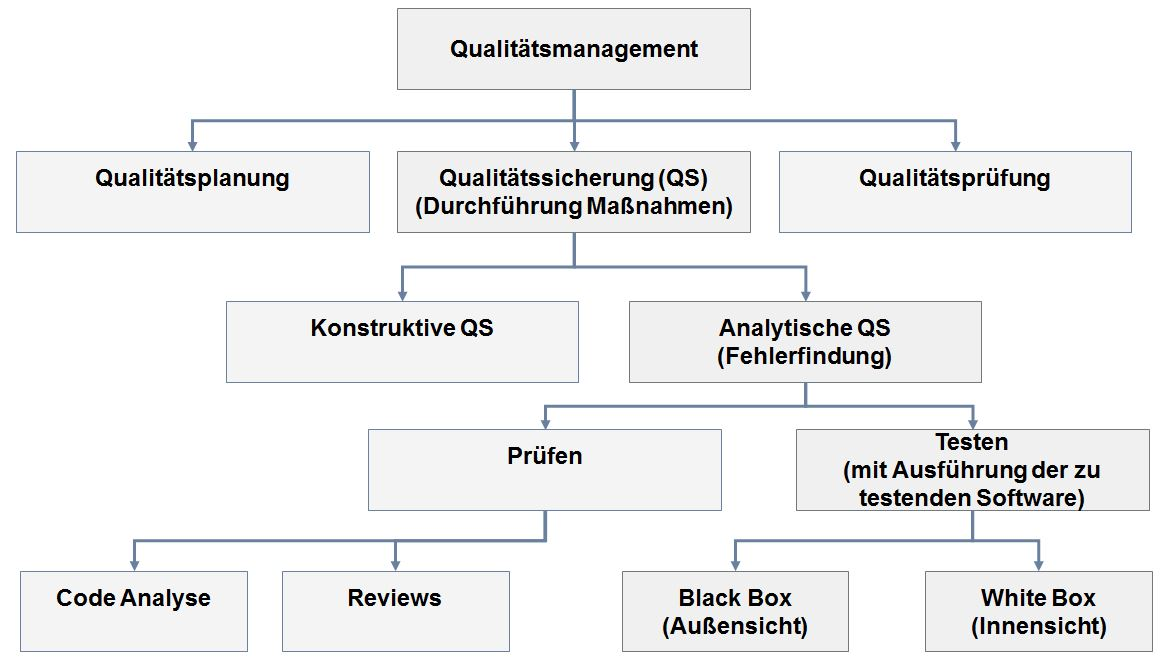
\includegraphics[scale=0.5]{img/qs.jpg}
	\captionof{figure}{\label{abb:sonarqube}Einordnung von SonarQube}
	\vspace{2em}
\end{minipage}




\section{Qualitätsmerkmale von Software}

Um die Qualität von Software bewerten zu können, wurden verschiedene Merkmale festgelegt, welche ausschlaggebend sind. Diese sind nach ISO 25010 genormt. Demnach sind zum Beispiel Faktoren wie Funktionalität, Zuverlässigkeit, Gebrauchstauglichkeit, Sicherheit und Effizienz entscheidend, um die Qualität der Software beurteilen zu können \autocite[Vgl.][]{Merkmale}.

Die Autoren des Buchs \enquote{SonarQube in action} beleuchten dieses Thema ebenfalls sehr umfassend. Sie bewerten die Qualität einer Software nach den sogenannten \enquote{Seven axes of code quality}\autocite[S.13]{SonarInAction}, nach dessen Maßstäben SonarQube geschriebenen Programmcode untersucht. 
Diese Achsen, auch \enquote{Seven Deadly Developer Sins}\autocite[S.13]{SonarInAction} genannt, beinhalten folgende Punkte: Potenzielle Bugs, Programmierrichtlinien, Tests, Duplikationen, Kommentare, Architektur und Design, sowie Komplexität.
Um alle Punkte abdecken zu können, sind die Regeln von SonarQube, anhand derer die Qualität einer Software bemessen wird, auf diese sieben Achsen abgestimmt.

